% CSA processing flow figure (TikZ).
% Coordinates in drawio-style px (1 unit = 0.02 cm, y pointing down). Requires tikz.
% Usage: \resizebox{<width>}{!}{% CSA processing flow figure (TikZ).
% Coordinates in drawio-style px (1 unit = 0.02 cm, y pointing down). Requires tikz.
% Usage: \resizebox{<width>}{!}{% CSA processing flow figure (TikZ).
% Coordinates in drawio-style px (1 unit = 0.02 cm, y pointing down). Requires tikz.
% Usage: \resizebox{<width>}{!}{% CSA processing flow figure (TikZ).
% Coordinates in drawio-style px (1 unit = 0.02 cm, y pointing down). Requires tikz.
% Usage: \resizebox{<width>}{!}{\input{../figures/pipeline/csa_flow.tex}}
% Blocks are drawn as fixed rectangles so adjacent blocks always share an edge.
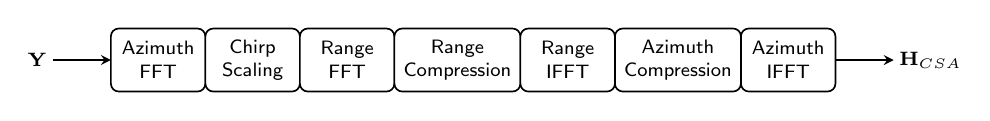
\begin{tikzpicture}[
    x=0.02cm, y=-0.02cm,
    font=\fontsize{7}{8.5}\linespread{1}\selectfont\sffamily,
    line width=0.6pt,
    lbl/.style={align=center, inner sep=0pt},
    flow/.style={-stealth},
  ]
  % Blocks: {left x / width / label}
  \foreach \x/\w/\t in {280/60/{Azimuth\\FFT}, 340/60/{Chirp\\Scaling}, 400/60/{Range\\FFT},
                        460/80/{Range\\Compression}, 540/60/{Range\\IFFT},
                        600/80/{Azimuth\\Compression}, 680/60/{Azimuth\\IFFT}} {
    \draw[rounded corners=1mm, fill=white] (\x,240) rectangle ++(\w,40);
    \node[lbl] at (\x+\w/2,260) {\t};
  }

  % Input and output
  \node[lbl, anchor=east] at (240,260) {$\mathbf{Y}$};
  \node[lbl, anchor=west] at (780,260) {$\mathbf{H}_{CSA}$};
  \draw[flow] (243,260) -- (280,260);
  \draw[flow] (740,260) -- (777,260);
\end{tikzpicture}
}
% Blocks are drawn as fixed rectangles so adjacent blocks always share an edge.
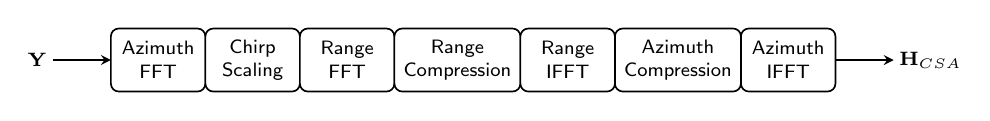
\begin{tikzpicture}[
    x=0.02cm, y=-0.02cm,
    font=\fontsize{7}{8.5}\linespread{1}\selectfont\sffamily,
    line width=0.6pt,
    lbl/.style={align=center, inner sep=0pt},
    flow/.style={-stealth},
  ]
  % Blocks: {left x / width / label}
  \foreach \x/\w/\t in {280/60/{Azimuth\\FFT}, 340/60/{Chirp\\Scaling}, 400/60/{Range\\FFT},
                        460/80/{Range\\Compression}, 540/60/{Range\\IFFT},
                        600/80/{Azimuth\\Compression}, 680/60/{Azimuth\\IFFT}} {
    \draw[rounded corners=1mm, fill=white] (\x,240) rectangle ++(\w,40);
    \node[lbl] at (\x+\w/2,260) {\t};
  }

  % Input and output
  \node[lbl, anchor=east] at (240,260) {$\mathbf{Y}$};
  \node[lbl, anchor=west] at (780,260) {$\mathbf{H}_{CSA}$};
  \draw[flow] (243,260) -- (280,260);
  \draw[flow] (740,260) -- (777,260);
\end{tikzpicture}
}
% Blocks are drawn as fixed rectangles so adjacent blocks always share an edge.
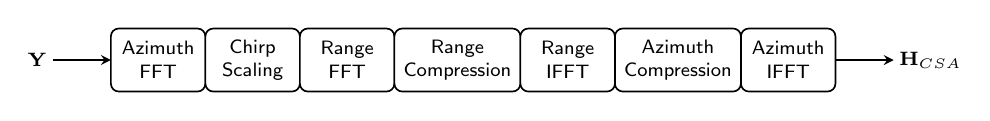
\begin{tikzpicture}[
    x=0.02cm, y=-0.02cm,
    font=\fontsize{7}{8.5}\linespread{1}\selectfont\sffamily,
    line width=0.6pt,
    lbl/.style={align=center, inner sep=0pt},
    flow/.style={-stealth},
  ]
  % Blocks: {left x / width / label}
  \foreach \x/\w/\t in {280/60/{Azimuth\\FFT}, 340/60/{Chirp\\Scaling}, 400/60/{Range\\FFT},
                        460/80/{Range\\Compression}, 540/60/{Range\\IFFT},
                        600/80/{Azimuth\\Compression}, 680/60/{Azimuth\\IFFT}} {
    \draw[rounded corners=1mm, fill=white] (\x,240) rectangle ++(\w,40);
    \node[lbl] at (\x+\w/2,260) {\t};
  }

  % Input and output
  \node[lbl, anchor=east] at (240,260) {$\mathbf{Y}$};
  \node[lbl, anchor=west] at (780,260) {$\mathbf{H}_{CSA}$};
  \draw[flow] (243,260) -- (280,260);
  \draw[flow] (740,260) -- (777,260);
\end{tikzpicture}
}
% Blocks are drawn as fixed rectangles so adjacent blocks always share an edge.
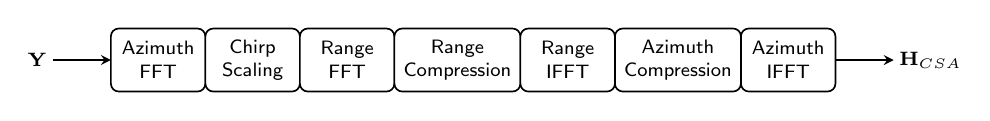
\begin{tikzpicture}[
    x=0.02cm, y=-0.02cm,
    font=\fontsize{7}{8.5}\linespread{1}\selectfont\sffamily,
    line width=0.6pt,
    lbl/.style={align=center, inner sep=0pt},
    flow/.style={-stealth},
  ]
  % Blocks: {left x / width / label}
  \foreach \x/\w/\t in {280/60/{Azimuth\\FFT}, 340/60/{Chirp\\Scaling}, 400/60/{Range\\FFT},
                        460/80/{Range\\Compression}, 540/60/{Range\\IFFT},
                        600/80/{Azimuth\\Compression}, 680/60/{Azimuth\\IFFT}} {
    \draw[rounded corners=1mm, fill=white] (\x,240) rectangle ++(\w,40);
    \node[lbl] at (\x+\w/2,260) {\t};
  }

  % Input and output
  \node[lbl, anchor=east] at (240,260) {$\mathbf{Y}$};
  \node[lbl, anchor=west] at (780,260) {$\mathbf{H}_{CSA}$};
  \draw[flow] (243,260) -- (280,260);
  \draw[flow] (740,260) -- (777,260);
\end{tikzpicture}
